\subsection{CSTMD1}

A C++/Cuda simulator, which has been wrapped in Cython, has been developed that can model several mutually inhibiting multi-compartmental neurons using the Hodgkin-Huxley mathematical. The simulator successfully models spike propagation from the dendritic tree \cite{CSTMD1} to the soma although it can overflow due to the model's sensitivity to its time step.

Simultaneously modelling several thousand differential equations has a significant computation overhead. Therefore if the simulation pipeline is to run near real-time (requirement B5 Table \ref{table:req}) the performance of the CSTMD1 simulator is critical. Therefore NVIDIA libraries were used including cuBLAS which contains highly optimised linear algebra subroutines. Table \ref{table:cstmd_performance} shows the current average computation of the simulator for varying numbers of compartments and electrodes. There is  small increase in GPU computation time (a primary reason for using the CUDA platform) and a large increase in overall execution time attributable to the relatively slow process of copying data to and from GPU memory. As such only the minimal amount of data will be copied back onto host memory.

\begin{table}[!ht]
    \centering
    \begin{tabular}{c|c|c|c}
    Compartments & Electrodes &  Avg GPU Computation /ms  & Avg Total Time /ms  \\\hline
    10 & 4 & 1.17 & 2.87     \\
    2000 & 35 & 1.25 & 26.2  \\
    7500 &50 & 1.30 & 41.2  \\
    \end{tabular}
    \caption{Time to simulate 1ms. \textit{Avg GPU Computation} is the time to simulate 1ms in pure GPU computation, \textit{ Avg Total-Time} is the time to execute one step from the Python wrapper and includes the overhead of retrieving the electrode data from the GPU memory and transforming it into a Python data structure (GPU time step = 0.05ms)}
    \label{table:cstmd_performance}
\end{table}

In order to better understand the module's characteristics (see requirement B1, Table \ref{table:req}), a ``Neuron Visualiser" (Figure \ref{fig:neuron_visualiser}) has been developed which generates a 3D model of a collection of neurons and animates the propagating spikes. This will help in observing the effect of the morphology and inhibition on the performance of the simulator.

\begin{figure}[!ht]
    \centering
    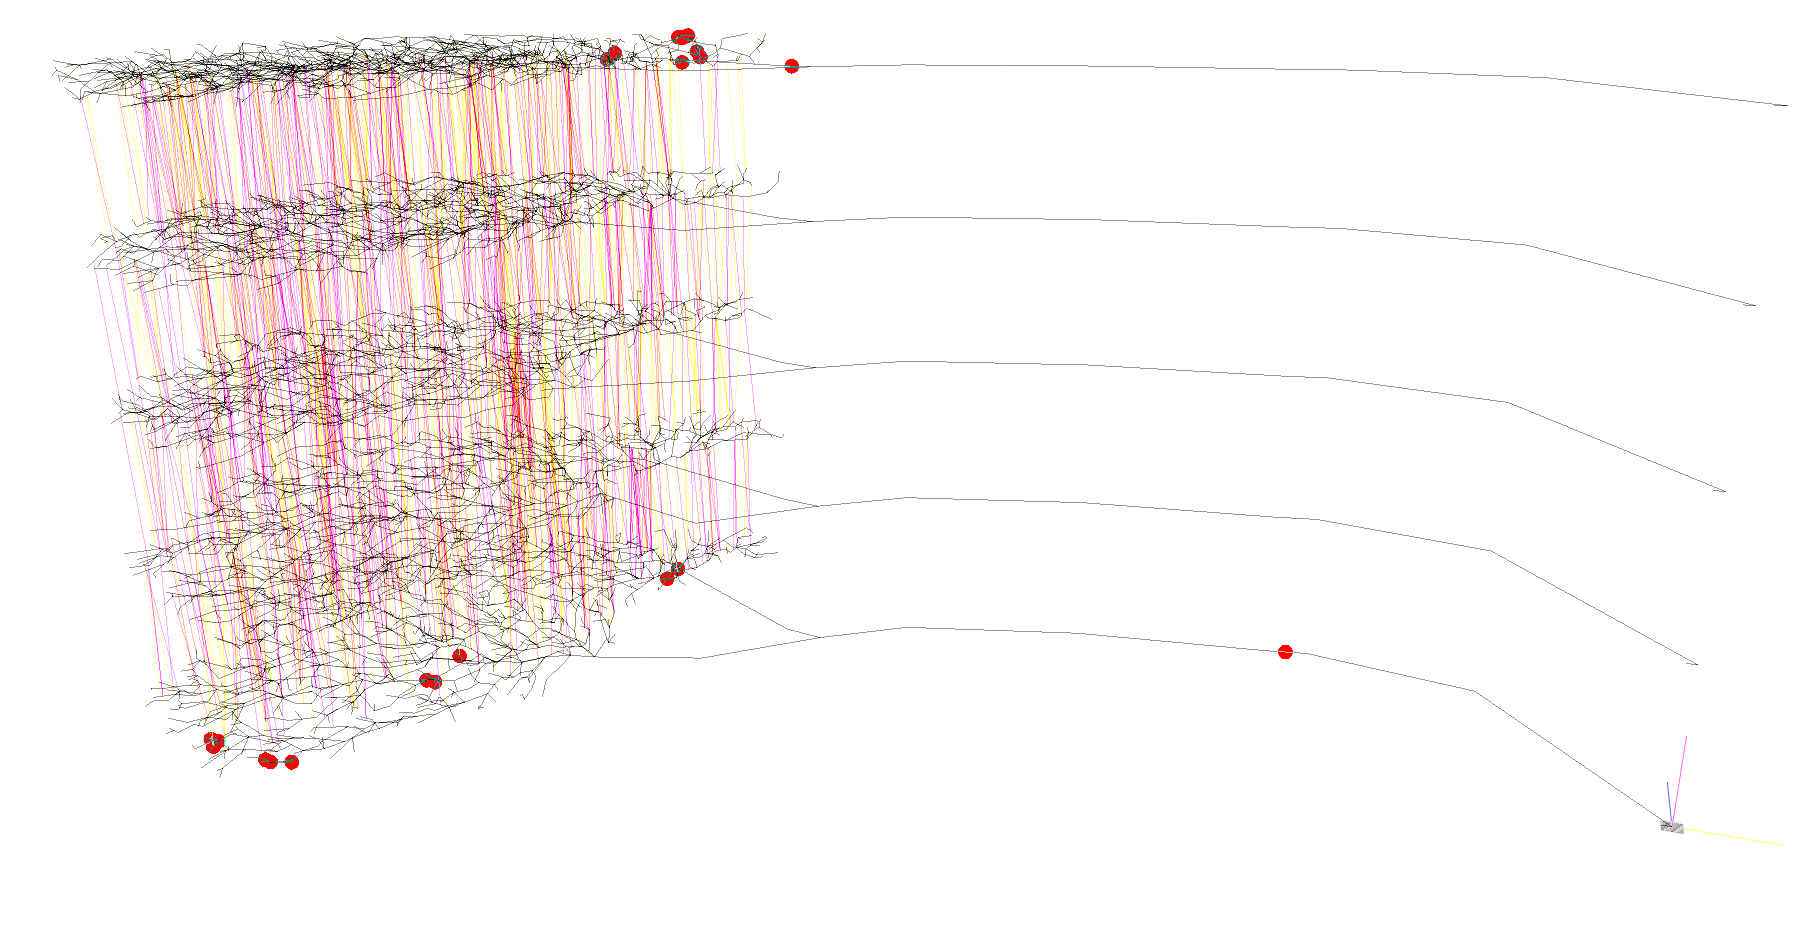
\includegraphics[width = 0.65\textwidth]{Figures/neuronvisualiser2.png}
    \caption{CSTMD1 network, 5 neurons, 7500 compartments viewable using the Neuron Visualiser}
    \label{fig:neuron_visualiser}
\end{figure}

We will conduct model verification in order to tune the parameters to observe the bi-stability required for successful target selection. It is also possible to enrich the neuron model with individual compartment parameters and a topological mapping of the ESTMD stimulus, however the group's focus will remain on integration and model verification.

